% "Станет проще"

\documentclass[a4paper,12pt]{article} % тип документа

% report, book

% Рисунки
\usepackage{graphicx}
\usepackage{wrapfig}

\usepackage{hyperref}
\usepackage[rgb]{xcolor}



%  Русский язык

\usepackage[T2A]{fontenc}			% кодировка
\usepackage[utf8]{inputenc}			% кодировка исходного текста
\usepackage[english,russian]{babel}	% локализация и переносы


% Математика
\usepackage{amsmath,amsfonts,amssymb,amsthm,mathtools} 


\usepackage{wasysym}

%Заговолок
\author{Сафиуллин Роберт	}
\title{Лабортаорная работа 2.5.1}





\begin{document} % начало документа

\maketitle


\newpage
\section{Цель работы:}
1)  Экспериментально выявить участок сформированного течения, определить режимы ламинарного и турбулентного течения; определить число Рейнольдса.\\
\section{В работе используются:}
Металлические трубки, укрепленные на горизонтальной подставке; газовый счетчик; микроманометр типа ММН; стеклянная U-образная трубка; секундомер.
 \section{Описание работы}
 Рассмотрим движение вязкой жидкости или газа по трубке круглого сечения. При малых скоростях потока движение оказывается ламинарным (слоистым), скорости частиц меняются по радиусу и направлены вдоль оси трубки. С увеличением скорости потока движение
становится турбулентным, и слои перемешиваются. При турбулентном движении скорость в каждой точке быстро меняет величину и направление, сохраняется только средняя величина скорости.

Характер движения газа (или жидкости) в трубке определяется безразмерным числом Рейнольдса: $$Re=\frac{vrp}{\eta}$$

В гладких трубах круглого сечения переход от ламинарного движения к турбулентному происходит при Re ≈ 1000.

При ламинарном течении объем газа V, протекающий за время t по трубе длиной l (называемый расходом), определяется формулой Пуазейля: $$Q_V=\frac{\pi r^4}{8l\eta}(P_1-P_2)$$
При	втекании	газа	в	
трубку	из большого резервуара скорости слоев вначале постоянны по всему сечению (рис. 1). 
\indent
\indent По мере продвижения  газа по	трубке	
картина распределения скоростей меняется, так как сила трения о стенку тормозит прилежащие к ней слои. Характерное для ламинарного	
течения параболическое распределение скоростей устанавливается на	
некотором расстоянии a от входа в трубку, которое зависит от радиуса трубки r и числа Рейнольдса по формуле: $$a\approx0,2r*Re$$.\\
\newpage
\section{Экспериментальная установка:}
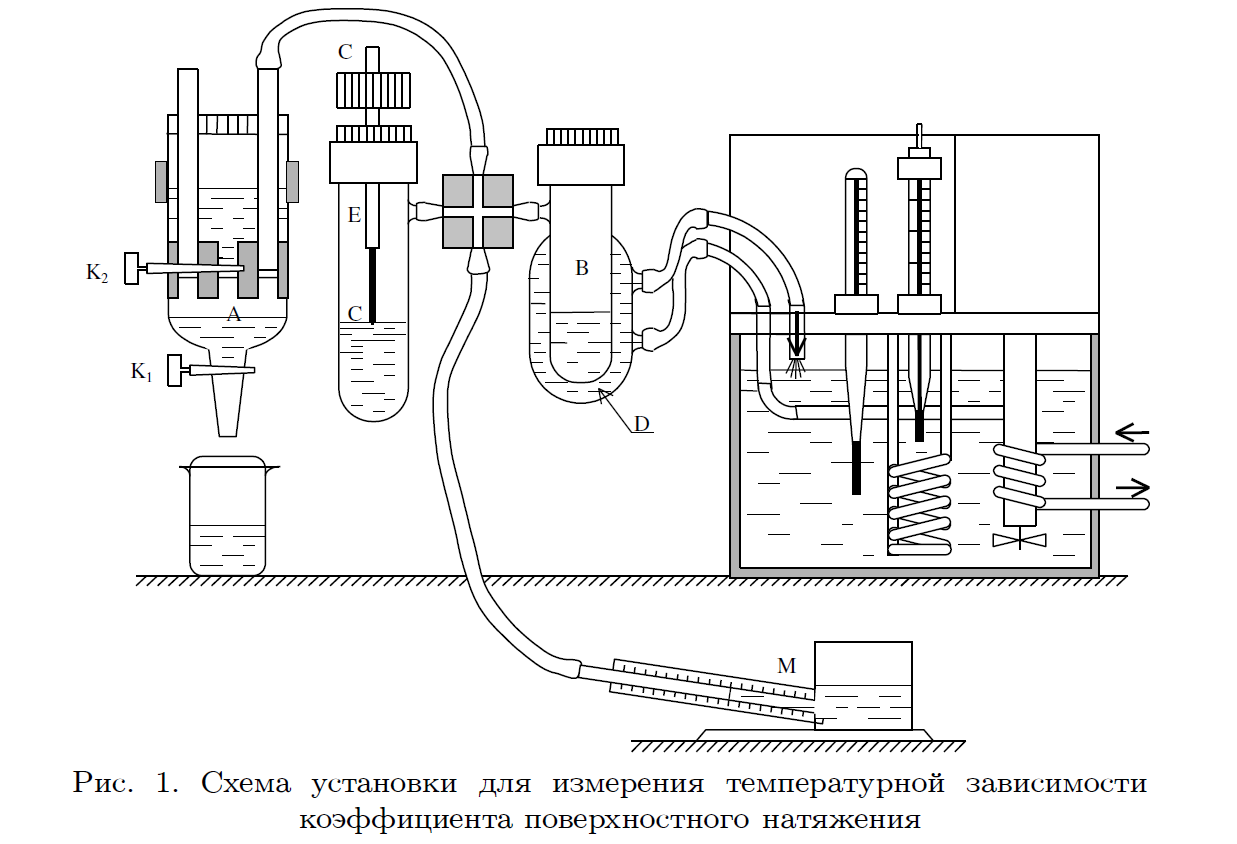
\includegraphics[scale=0.7]{ust}
 Обычно кончик иглы лишь касается поверхности жидкости, чтобы исключить влияние гидростатического давления столба жидкости. Однако при измерении температурной зависимости коэффициента поверхностного натяжения возникает ряд сложностей. Во-первых, большая теплопроводность металлической трубки приводит к тому, что температура на конце трубки заметно ниже, чем в глубине жидкости. Во-вторых, тепловое расширение поднимает уровень жидкости при увеличении температуры. Это гидростатическое давление вычитается из падения лапласова давления вследствие уменьшения $\sigma$, и в опыте с анилином, например, наблюдаемый эффект меняет знак при высоте столба жидкости порядка пяти сантиметров. Обе погрешности можно устранить, погрузив кончик трубки до самого дна. Полное давление, измеренное при этом микроманометром, $P = \Delta P + \rho gh $, где последний член определяется только массой воды.\\
\ \\
Давление P вычисляется с помощью показаний манометра N в у.е по формуле:

$$P=0.2*9.80665*N$$
$\sigma=22.8*10^{-3}$ Н/м - коэффициент поверхностного натяжения спирта\\
$\gamma = 0.8095$ г/см$^3$ - плотность спирта
\section{Ход работы}
1) Оценим диаметр иглы. Для этого измерим давление пробулькивания, когда игла находится на поверхности спирта. Оно олучилось равным:

$$P=0.2*9.80665*39=76.5 Pa$$

Тогда $d=4\sigma/P\approx 1.19$ мм. Прямые замеры с помощью микроскопа дали значения 1.2$\pm$0.2 мм 

Примем диаметр иглы равным 1.2$\pm$0.2 мм

2) Теперь утопим иглу до предела. При этом замерим $h_1$ и $h_2$ на поверхности и на глубине соответственно а также показания манометра.

Получили:
$h_1$=3.4$\pm$0.05 cm

$h_2$=0.7$\pm$0.05 cm

Отсюда рассчитаем $\triangle$P по формуле $\rho$g$\triangle$h:

$\triangle$P=134.86$\pm$4 Pa

А также зная, что показания манометра у дна равны 90$\pm$2 у.е, рассчитаем  $\triangle$$P_M$=98.06$\pm$3.9 Pa

3) Теперь поместим иглу в пробирку с водой и начнем нагревать ее, при этом снимая зависимость $\sigma$(T). Параллельно рассчитаем:

$q=-T\frac{d\sigma}{dT}$ - теплота образования единицы площади \\

$U_\Pi = (\sigma-T\frac{d\sigma}{dT})\Pi$ - поверхностная энергия единицы площади\\

Результаты запишем в таблицу:

\begin{tabular}{|c|c|c|c|c|c|c|}
\hline 
T, K & 300.1 & 305.1 & 310.1 & 315.1 & 320.1 & 325	.0 \\ 
\hline 
N, у.е & 185 & 184 & 183 & 181 & 180 & 179 \\ 
\hline 
$\sigma*10^{-3}$ Н/м  & 218 & 217 & 215 & 213 & 212 & 211 \\ 
\hline 
$q*10^{-3}$ Н/м  & 90.03 & 91.53 & 93.03 & 94.53 & 96.03 & 97.5 \\ 
\hline 
$U_\Pi / \Pi*10^{-3}$ Н/м & 308.03 & 308.53 & 308.03 & 307.53 & 308.03 & 307.5 \\ 
\hline 
\end{tabular} \\

4) По этим данным построим графики $\sigma (T)$, $q (T)$ и $U_\Pi/\Pi (T)$ в одной координатной плоскости

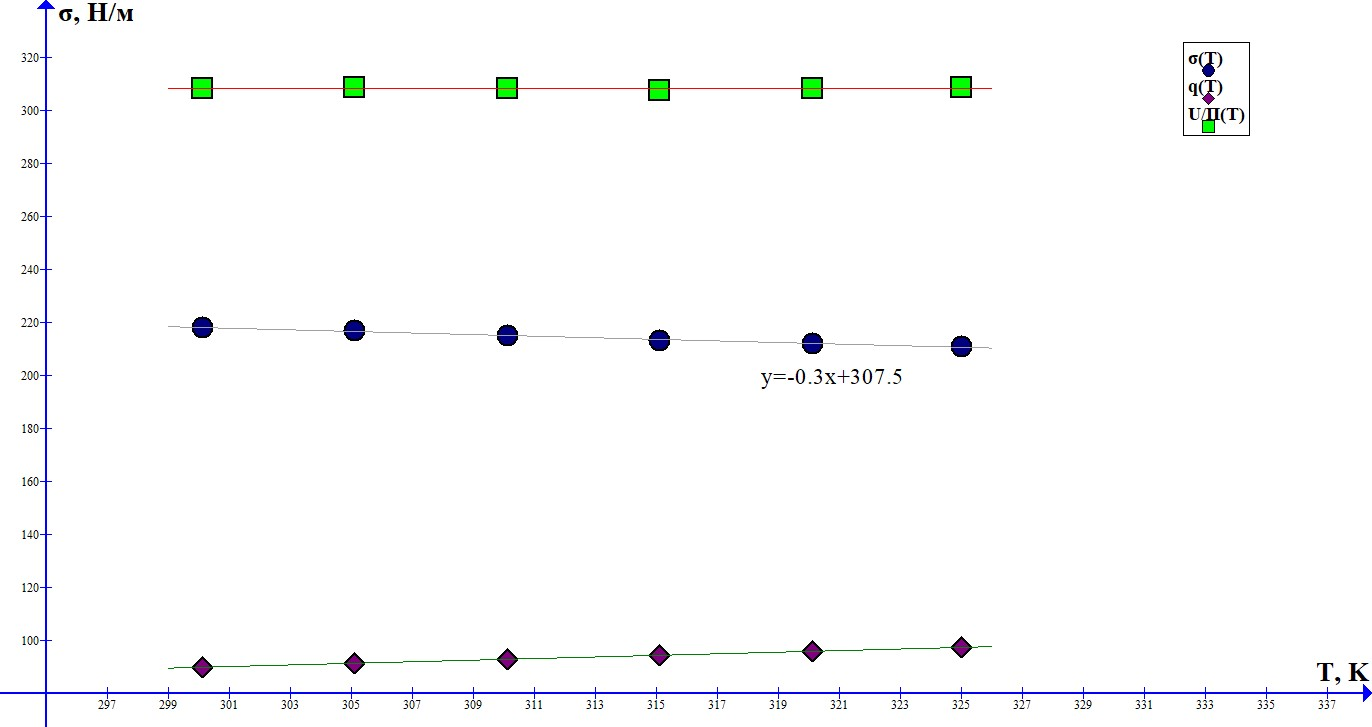
\includegraphics[scale=0.34]{2511}


Таким образом графики подтвержадют линейность $\sigma (T)$, $q (T)$ и $U_\Pi/\Pi (T)$ и убывание $\sigma$ с увеличением температуры.



















\end{document} % конец документа